\documentclass{acm_proc_article-sp}
\usepackage{color}
\usepackage{listings}
\lstset{breaklines=true, basicstyle=\scriptsize, frame=single, 
  keywordstyle=\color{blue}, commentstyle=\color{green},
  identifierstyle=\color{cyan},
  stringstyle=\ttfamily\color{red}, showstringspaces=false,
  language=Java, numberfirstline=true,
  frameround=true, frame=trBL}
\title{Specifying and Detecting Meaningful Changes in Programs}
\author{
   \begin{tabular}{c}
   Yijun Yu \\
   Computing Department, The Open University, United Kingdom
   \end{tabular}
}
\newtheorem{definition}{Definition}
\begin{document}
\maketitle
\begin{abstract}
Not all changes kept in software repositories are essential. In this work we devise an automated technique to specify, for programs of domain-specific languages, which kinds of changes are considered meaningful to the detectives. Such specifications are lightweight extension of existing grammars to enable an efficient implementation of change detections with a small effort. Our technique has been evaluated with respect to performance and scalability, on a benchmark of programs in comparison to similar techniques. 
\end{abstract}
\section{Introduction}

``Nothing endures but change.'' -- Heraclitus (c.535 BC - 475 BC). This philosophy is largely true in any software development project.
However, not all changes are equally meaningful to different people. For example, the activities of changing the indentations of statements do not necessarily change the meanings or semantics expressed by the program. Nonetheless they could cause false alarms by any revision control system through text-based difference comparison algorithms (e.g., the {\bf diff} utility in Unix). Although such indentations are not meaningful to the executation of C/Java programs, they can be meaningful to programs in other programming languages such as Python, and can also be meaningful to C/Java developers who care about pretty prints for the maintenance. Similarly, graphs used in requirements/design modeling activities typically allow moving nodes around in order to present the model in a different physical layout, whilst the topology is preserved. Often such layout changes are saved through the serialisation, leading to false alerts that the software design has changed. 

These are just a few examples of how important and challenging it is to detect meaningful changes. The general problem remains the same. Given that a change considered meaningful to someone may be meaningless to others, and vice versa, how can people or software engineering tools be informed appropriately to ignore or detect such a change? Some difference comparison tools can be {\em customized} to detect different kinds of changes, e.g., {\tt diff} either accepts or rejects whitespace differences depending on whether or not a command line switch {\tt -w} has been used. Such choices, however, can be misused easily by programmers who, for example, accept whitespaces changes in Python programs, or reject those in Java programs. Specific to the needs of programmers, it is often the case that whitespaces within one region of the program require attention while those within another are irrelevant. A global choice made for the {\tt diff} command is inappropriate in such cases. 

In this paper, we propose a new way to specify meaningful changes as materialised views to various artifacts including requirements models, UML diagrams and programming languages. Such specific views are defined declaratively as a lightweight extension to the grammar of the subject languages. We design the extension as a few generic modifications to the meta-grammar\footnote{The grammar of a TXL grammar is expressed in TXL too.} of TXL~\cite{txl} such that it is applicable to any language specifiable by TXL, which includes general-purpose programming languages (e.g., C/Java/Python) as well as graphical modeling languages (e.g., EMF, XMI, GXL). The extended grammar is {\em bootstrapped} into an on-the-fly {\em normalisation} transformation that removes meaningless differences from the concrete programs. These outputs of normalised programs are pretty-printed automatically for other text-based difference detection tool, as simple as {\tt diff}, to detect the meaningful differences.

To evaluate the versatility and efficiency of our meaningful changes extension to TXL (hereafter {\tt mct}), we show the results of two sets of experiments. The first set of experiments demonstrate how much changes are required to specify meaningful changes on different programming languages, ranging from i*/{\em Problem Frames} for requirements models, UML class diagrams for designs and C/Java/Python programming languages. The second set of experiments compare its efficiency with related {\tt diff} tools in detecting changes in the evolution of the {\tt JHotDraw} project.  
   
The remainder of the paper is organised as follows: Section~\ref{sec:background} introduces two small examples as running examples to illustrate the problem and the requirements for specifying and detecting meaningful changes. Section~\ref{sec:approach} explains the approach we adopt to bootstrap the normalisation transformations needed in the implementation of the tool. %, which is illustrated by the running example in Section~\ref{sec:example}.
Section~\ref{sec:experiment} presents the results of a number of experiments in using the tool, and comparing them with existing {\tt diff} tools for versatility and efficiency. Section~\ref{related} brings up the comparision of the conceptual differences in the design of the different approaches, and indicates some limitations of our approach. Section~\ref{conclude} concludes the findings in this work.

\section{Motivating Examples}\label{sec:background}
A program is considered meaningfully different from another only when it has non-trivial changes; otherwise it is considered meaningfully the same even after introducing trivial changes by, e.g., adding or deleting whitespaces, or by reordering the type modifiers in method declarations, etc. 
\subsection{Programs and {\tt diff / ldiff}}
The essence can be illustrated using a simple Java program in Listing~\ref{listing:1}.
\lstinputlisting[numbers=left,caption={\tt cat -n HelloWorld.java},label=listing:1]{code/HelloWorld.java}

It is still the same program even after a programmer modifies it into Listing~\ref{listing:2}.
\lstinputlisting[numbers=left,caption={\tt cat -n HelloWorld2.java},label=listing:2]{code/HelloWorld2.java}
Traditional comparison tool such as the Unix {\tt diff} utility reports a number of trivial changes (Listing~\ref{listing:3}), e.g.,
an insertion of the declaration of the {\tt world} string (the Lines 3-4 chunk of HelloWorld2.java) and the replacement of the chunk of HelloWorld.java (Lines 4-6) with the chunk of HelloWorld2.java (Lines 6-8).
%\lstinputlisting[caption={diff HelloWorld2.java HelloWorld.java},label=listing:3]{code/HelloWorld2.diff}
\lstinputlisting[language=,identifierstyle=,caption={\tt diff -w HelloWorld2.java HelloWorld.java},label=listing:3]{code/HelloWorld2-w.diff}
Applying a more advanced line-diffing algorithm {\tt ldiff}~\cite{canfora09software} to this example, one can see that 5 smaller hunks of changes are still reported as 2 insertions, 1 deletions and 2 modifications, even though they are now smaller for programmers to check.
\lstinputlisting[language=,identifierstyle=,caption={\tt ldiff.pl -w -o diff HelloWorld2.java HelloWorld.java},label=listing:ldiff]{code/HelloWorld3-w.diff}

In fact, none of the changes identified in this example is meaningful if the programmer only wants to see non-trivial
changes: just as adding a newline or some whitespaces would not change the syntax of the program, nor would swapping the keywords {\tt public} and {\tt static} in the declaration of the {\tt main} method make any semantic differences.

\subsection{Graphs and serialisation/abstraction}
Graph models have similar problems, if not worse. To illustrate this point, consider the two simple diagrams drawn by an Eclipse-based graphical modeling tool in Figure~\ref{fig:1}\footnote{Most UML modeling tools based on Eclipse also use the same underlying model-driven technology to create the editor plugins for editing and saving EMF/GMF models such as class diagrams.}.
Although the diagram below has changed the diagram above it by placing the ellipse node (Requirement) on the left rather than on the right, and by filling different colors into the shapes, the topology of the graph and the content of the corresponding EMF model remain the same, according to the domain-specific language defined in Problem Frames~\cite{jackson01}.
\begin{figure}
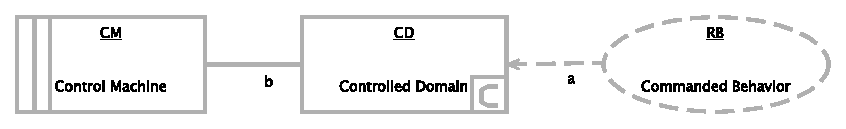
\includegraphics[width=\columnwidth]{code/CommandedBehaviour1}
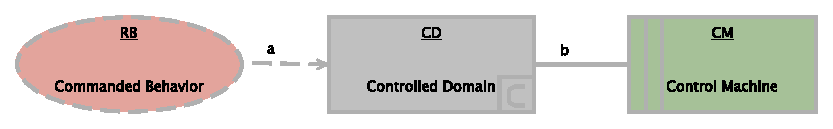
\includegraphics[width=\columnwidth]{code/CommandedBehaviour2}
\caption{Equivalent problem frame diagrams: commanded behaviour}\label{fig:1}
\end{figure}

The underlying {\tt HashMap} in the modeling tool, however, could serialise the modeling elements by different (and rather random) orderings, making it more difficult for a simple diff tool to detect meaningful changes to their EMF models. The EMF model can be saved as an equivalent model in corresponding domain-specific (textual modeling) language (DSL) such as those specified using the Eclipse Xtext framework~\footnote{http://eclipse.org/xtext} (e.g., List~\ref{listing:xtext}). 
 \lstinputlisting[language=,identifierstyle=,numbers=left,emph={problem,event},stringstyle=\color{red},caption={\tt cat -n CommandedBehaviour.problem},label=listing:xtext] {code/CommandedBehaviour1.problem}
Besides the whitespace problems, in this example, the phenomena are not alphabetically ordered, nor do the domain nodes. 
One can imagine easily that swapping two nodes or two phenomena in this serialised model could lead to false alarms which in fact do not require attention by the designers. Comparing two models at the EMF level using a tool such as {\tt EMFcompare}~\footnote{http://eclipse.org/emfcompare}, one could avoid such false alarms\footnote{TO CHECK}.

Moreover, analysts/designers do not always want to view every detail of the modeling elements. For example, the phenomena of the domain nodes in a problem diagram, or the exact declaration of the class methods in a class diagram, are not viewed when the analyst/designers is concentrating on the structural relationship between the larger entities (domain interfaces or class hiearchies). As such, an abstraction transformation is often required before one compare meaningful structures rather than the meaningless details that should be hidden from the view. Of course, programmers may sometimes want to compare the details of the exact declarations of method, while still would wish to ignore the detail implementation of the method bodies. Therefore for the same model (e.g., graph) it is helpful to allow an abstraction as the preprocessing step for a meaningful comparison.

\section{Bootstrapping Normalisation}\label{sec:approach}

Before explaining the theory and the implemenations of our transformations, we first define {\em normalisation transformations} and their rationale.
\begin{definition}
{\bf Normalisation (normalising transformation).\label{defn:norm}} A program $P$ is said to be {\tt normalised} into a program $N(P)$ if any program $P'$ such that $P'\neq P \wedge N(P') = N(P)$ is {\em meaningfully equivalent} to $P$. In other words, $N(P)$ is the representative element of the equivalent class to which $P$ belongs, and $P'$ has no meaningful changes to $P$.
\end{definition}
As discussed earlier, the exact meaning for `meaningful equivalent' in  the Definition~\ref{defn:norm} is intentionally left open or undefined because it depends on the purpose of the analysis. Even so, the definition is still useful because it provides the general criteria for determining whether a transformation is a suitable normalisation once it is clear what is meaningfully equivalent to the users. Once the normalisation transformation is defined, the detection of the meaningful changes becomes comparing the two normalised programs. However, in principle there are infinite possible normalisation transformations for some equivalent classes. For example, adding any number of whitespaces can be regarded as normalisation transformations. 
According to Definition~\ref{defn:norm2}, it is not possible to have infinite number of normalisations because the programs are of finite size.
\begin{definition}
{\bf Terminable Normalisation.\label{defn:norm2}} A normalisation $N$ is terminable if $N(P)$ is strictly smaller than $P$ in size.
\end{definition}

Although not mandatory, for pragmatic reasons it is preferable to have the outputs of normalisation readily compared by reusing line-based diff tools. 
\begin{definition}
{\bf Diff-friendly Normalisation.\label{defn:norm3}} A normalisation $N$ is diff-friendly, if any line in the normalised program $N(P)$ has at most one meaningful changes.
\end{definition}

Given that a program is expressed in programming languages consist of production rules~\cite{aho79}, our normalisation tool {\tt mct} needs to satisfy the following requirements, in order to handle those examples motivated in the previous section:
\begin{enumerate}
\item [R1] Ignore the trivial differences in optional or repetitive {\em terminals} in the production rules;
\item [R2] Ignore certain non-terminals in the rules according to the needs of further abstraction;
\item [R3] Ignore the ordering of the unordered collections by ordering them sequentially, such that two collections of the same set of elements are the same sequences;
\item [R4] Carry out the normalisation transformations on the fly, without any user intervention once the grammar rules are extended using the annotations for [R1], [R2] and [R3].
\item [R5] (optional) Occupy at east one line per non-terminal;
\item [R6] (optional) Make sure the normalised program is still a valid program in the original grammar.
\end{enumerate}

The requirement [R1] is sufficient to ignore all unnecessary non-terminals in the output program. Such normalisations help focus the comparison more on the abstract syntax rather than on the concrete syntax, because it is the abstract syntax that carries the meaning of the representation while the concrete syntax (reflected by the non-terminals) are merely the auxiliary tokens to parse. The default {\em unparse} functionality of TXL~\cite{txl} can already satisfy the requirement of removing extra whitespaces. To remove the extra non-terminals, we must introduce the ``ignore'' attribute to the type specification, such as {\tt [opt 'terminal \underbar{'ignore}] }. Requirement [R2] is similar to that of [R1], but now it is the non-terminals that are to be ignored for the abstraction purpose. 

Requirement [R3] is useful especially when users knows when a list or an array of literals (tokens and non-terminals) is in fact unordered (e.g., the type modifiers in Java, the phenomena in problem frames), therefore combinatory numbers of possible differences can be removed by ordering the elements in the same way. By default, we can use the serialised string of the literal and sort them in ascending ordering. Of course, such ordering can be made more flexible by allowing users to specify the appropriate ordering key/transformations. Examples of this extension are {\tt [ repeat X \underbar{ordered} ] } where the non-terminal X will be ordered in the normalised program; or {\tt [list X \underbar{ordered by Y}] } where the non-terminal X will be ordered by the comparison rule specified by {\tt Y(X)}. In other words, users can choose to order the elements in descending order, or by the ordering of a particular key field. 

Satisfying the requirement [R4] would allow the transformation from the program to a `simplified' grammar to be generated on the fly, appending additional transformation rules by either ignoring or ordering the literals that have been extended.  The implementation of [R4] is done through the technique of {\em bootstrapping}, that is, to reflectively annotate certain literals in the TXL meta-grammar using the {\tt ignore} and {\tt ordered by} extensions given that the TXL grammar itself is expressed in TXL as a meta-grammar. By processing each annotation in the context of the production rules, it produces a context-aware rule for the transformation on-the-fly. Then the annotations are stripped off by default, which produces a pure-TXL grammar without the annotations, while additional rules based on those removed annotations are combined together. This combined grammar specification is then used to parse the programs in the original language and produces the normalised programs. 

Optionally, requirement [R5] can be  enforced by inserting a new line directive  {\tt \underbar {[NL]}} to the end of each non-terminal literal in the production rules. Sometimes the normalised program does not have to be a valid program in the same grammar because removing the details may make the output no longer a valid program, therefore [R6] is the default preference applied if the user would like to preserve the program syntax as well. For example, the abstracted program is still in valid Java syntax by retaining the \{ \} braces while hiding the body of a Java method.

\subsection{A Running Example}\label{sec:example}
To illustrate the application of the approach laid out in the previous section, here we use the example of the problem frames syntax to illustrate the point. Listing~\ref{listing:problem0} selects to show three production rules of the original problem frames grammar. Lines 1-3 define a {\tt problem\_description} as an array of elements ({\tt E}); Lines 5-7 define each element to have an optional description of {\tt details}; and Lines 9-13 define the details by a list of comma separated {\tt phenomena} inside curly braces. 
\lstinputlisting[language=,identifierstyle=,numbers=left,caption={\tt cat -n problem.rules0.grm},label=listing:problem0]{code/problem.rules0.grm}
Since one does not care whether an element is before another element or not, the array of {\tt E}  is unordered. Similarly, the ordering of the phenomena list is unimportant to the meaning of the problem frames language. To specify the normalisation, one only has to insert the \underbar{ordered} at the end of the {\tt [repeat E+]} and {\tt [list phenomena]} respectively, as shown in Listing~\ref{listing:problem1}.
\lstinputlisting[language=,identifierstyle=,numbers=left,caption={\tt cat -n problem.rules1.grammar},label=listing:problem1]{code/problem.rules1.grm}
Furthermore, if one would like to normalise the elements by the descending order, a user-defined rule {\tt Small} can be added in Listing~\ref{listing:problem2}. This is just to illustrate how easy it is to customize the comparison function, in case one would like to define a different key or ordering for the structure to be normalised.
\lstinputlisting[language=,identifierstyle=,numbers=left,caption={\tt cat -n problem.rules2.grammar},label=listing:problem2]{code/problem.rules2.grm}
Of course, the user may choose to ignore certain information to further abstract the normalised structure, e.g., as indicated in Listing~\ref{listing:problem3}, the {\tt details} can be ignored by using {\tt ignore} at the end of the optional part {\tt [opt details]}. 
\lstinputlisting[language=,identifierstyle=,numbers=left,caption={\tt cat -n problem.rules3.grammar},label=listing:problem3]{code/problem.rules3.grm}
Note that using the above extensions after {\tt opt}, {\tt repeat} and {\tt list} parts, the normalised programs will still be valid for the original syntax.

\subsection{The implementation}
The meaningful change detection tool {\tt mct} is implemented completely as a TXL program. The first part of the implementation is an extension to the TXL's metagrammar {\tt txl.grm}. Listing~\ref{listing:extend} shows the extension to the existing {\tt typeSpec} rule and the addition of rules {\tt orderedBy} and {\tt ignored}.
\lstinputlisting[language=,identifierstyle=,numbers=left,caption={\tt cat -n grm1.grm},label=listing:extend]{code/grm1.grm}
 
The second part of the implementation is a specification of the normalisation transformations, simplified in Listing~\ref{listing:normalise}: we removed the very similar rules for eliminating {\tt ignore} annotations, and for producing rules from the {\tt [list X orderedBy]} annotations because they are very similar to that of eliminating the {\tt orderedBy} annotations, and to that of producting rules for the {\tt [repeat X orderedBy]}, respectively. 

TXL programs can be understood top-down from the back. Lines 50-71 specify how to generate the transformation rules {\tt Rules} on the fly by checking every {\tt defineStatement} in the TXL grammar such as those definitions in Listings~\ref{listing:problem1} to~\ref{listing:problem3}.  For each occurrence of {\tt [repeat X ordered by F]}, the transformation in Lines 12-35 is invoked to generate a rule such as those instantiated in Lines 26-31. These rules have unique name because there names are constructed uniquely from the names of the {\tt defineStatement} and {\tt X}. By the end of the main transformation, the rule in Lines 2-10 are applied to eliminate the extended annotations introduced earlier by the rules in the Listing~\ref{listing:extend}. 
\lstinputlisting[language=,identifierstyle=,numbers=left,caption={\tt cat -n grm.Txl},label=listing:normalise]{code/grm2.grm}
\subsection{Generated normalisation transformation}
The above generic implementation is done on the meta-grammar of TXL. When it is applied to a concrete TXL grammar, such as the one specified by Listings~\ref{listing:problem1} to~\ref{listing:problem3}, a concrete normalisation transformation is produced in the original syntax of TXL, as shown in Listing~\ref{listing:output}. Lines 1-10 are the same as the original rules in the Listing~\ref{listing:problem0} because of the elimination rules. The user-defined comparison rule is retained as lines 11-16. 
The lines 17-21 and lines 22-28 are respectively generated from the context of the two {\tt orderedBy} annotations from Listing~\ref{listing:problem1}. Lines 17-21 uses the user-defined comparison rule because the {\tt orderedBy} has explicited specified the name of the rule {\tt Small}, lines 22-28 on the other hands use the default string comparison rule using the TXL's builtin rule {\tt $>$}. Another minor difference is that Lines 17-21 are for arrays {\tt repeat} whilst Lines 22-28 are for comma separated lists. Both of these generated rules {\tt normalise\_repeat\_problem\_description\_E} and {\tt normalise\_list\_details\_phenomena} are used by the generated {\tt main} rule to produce the normalised program {\tt Prg}. 

\lstinputlisting[language=,identifierstyle=,numbers=left,caption={\tt cat -n problem.Txl},label=listing:output]{code/problem.Txl}

In brief, the problem frames grammar has got 3 annotations inserted by the user, plus 1 additional user-defined string comparison rule for sorting the nodes in inverse alphabatical order. Similarly, we have annotated 11 repeat/list patterns in
the Java5 TXL grammar {\tt java.grammar} without introducing any user-defined ordering rules to accept the ascending alphabatical order by default. These 11 {\tt ordered} annotations already make a big difference for detecting meaningful changes.
\subsection{The normalised programs}
From Listing~\ref{listing:xtext}, applying the transformation in Listing~\ref{listing:output}, the normalised program is shown in Listing~\ref{listing:result} where the elements are descending alphabetically, while the phenomena are ascending alphabetically.
\lstinputlisting[language=,identifierstyle=,numbers=left,caption={\tt cat -n CommandedBehaviour.n1.problem},label=listing:result]{code/CommandedBehaviour.normalised.problem}
Alternatively when the {\tt [opt details ignored]} is specified, Listing~\ref{listing:result2} shows the resulting abstraction where the details are ommitted.
\lstinputlisting[language=,identifierstyle=,numbers=left,caption={\tt cat -n CommandedBehaviour.n2.problem},label=listing:result2]{code/CommandedBehaviour2.normalised.problem}
As long as the same normalisation is used, two programs with meaningfully changes will be detected while the opposite will not.

Applying the same generic {\tt mct} transformation to the two Java programs in Listings~\ref{listing:1} and~\ref{listing:3} are now normalised into the same program in Listing~\ref{listing:result3}. Both {\tt hello} and {\tt world} members are ordered after the {\tt main} method by the alphabetical ordering;  {\tt public} and {\tt static} are also ordered in the same way. These normalisation would no longer differentiate the variations in the Listings~\ref{listing:1} and~\ref{listing:3}.
\lstinputlisting[numbers=left,caption={\tt txl HelloWorld.java java.grammar\\txl HelloWorld2.java java.grammar },label=listing:result3]{code/HelloWorld3.java}

\section{Evaluation}
In this section, we aim to evaluate the proposed {\tt mct} tool for the efficiency and scalability to normalise programs.
%\subsection{Versatility: The annotations on TXL grammars}
%Out of the default TXL installation~\cite{txl}, there are about a dozen grammars for various programming languages.
%As we are learning TXL, several of our own TXL languages are developed as well. 
Table~\ref{table:2} lists the grammars with the number of meaningful annotations as well.

\begin{table}
\caption{Size of the full grammar extended\label{table:2}}
\begin{tabular}{| r || r | r | r | r | }\hline
{\bf Grammar} & description & LOC & +LOC \\  \hline\hline
txl.grm & TXL meta-grammar & 408 & 15 \\ \hline
java.grm & Java 5 &  979 &  11 \\ \hline
%pyindent.grm & Python & 228 & \\ \hline
problem.grm &  problem frames & 82 & 5 \\ \hline
%json.grm & JSON format for Javascript & 36 & \\ \hline
%yaml.grm & YAML serialisation format & 94 & \\ \hline
%uncal.grm & UNQL+ format & 111  & \\\hline
%q7.grm & i* requirements &  100 & \\\hline
%argument.grm & Argumentation & 41 & \\\hline
%dot.grm & Graphviz directed graph & 79 & \\\hline
%ec.grm & Event calculus &  41 & \\\hline
\hline\end{tabular}
\end{table}

%\subsection{Efficiency: The evolution of JHotDraw code}
To evaluate the efficiency of {\tt mct}, we take the CVS repository of {\tt org.eclipse.gmf} modeling project, fetched on April 15, 2011. First, we checkout every single revision of every RCS file with the extension of {\tt ,v}. Then we compare every consequent files by the {\tt diff}, {\tt ldiff} and {\tt mct} commands. If the differences are non-empty, we count the number of revisions,  number of non-empty differences and the time it took to compute the results.
\begin{table}\centering
\caption{Performance of change detction\label{table:2}}
\begin{tabular}{| r || r | r | r | r ||}\hline
{\bf GMF} &  {\bf cmts} & {\bf Rev.} & {\bf Hunks} & {\bf Time} \\\hline\hline
{\tt diff} & with & 17,521 & 93,254 & \\\hline
{\tt   + diff} & w/o & 15,116 & 41,212 & \\\hline
{\tt ldiff} & with &  & & \\\hline
{\tt txl + ldiff} & w/o  &  & & \\\hline
{\tt mct + diff} &w/o  & & & \\\hline
{\tt mct + ldiff} &w/o  & & & \\\hline
\hline\end{tabular}
\end{table}

\section{Related work}
\subsection{Grammarware}
 
   ~\cite{klint05tosem}
   
\subsection{Transformation systems}

   `TXL` [cordy02]
   
\subsection{Bi- Directional Synchronisation}

   `UnQL+`
   
\subsection{Model- Driven Development}

   `Kermeta`, `ATL`
   
\subsection{Requirements Traceability}

   Information Retrieval
   
\subsection{Change Management}

   `CVS`, `Subversion`
   
   `Git`
   
\subsection{Fine- grained Change Management}

   `Molhado`
   
   Incremental IR
   
\subsection{Invariant Traceability}

   RE05, ICSM08, ASE08
   
\subsection{Model Diff}
\section{Conclusions and future work}

   Scalability
   
   Meta-changes: Changes to the Transformations
   
   We believe there is no need for infinite meta-levels. One example is `KM3` or `MOF`, although in principle there is always a possibility to ask for meta-level 
   changes, typically the language is less likely to change than the program.
   
   How to make use of `iChange` for runtime adaptation?
   
   The deployed system also need to adapt dynamically to the changes in its environment at runtime.
\cite{klint05tosem}  
\cite{cordy02} 
\cite{txl} 
\cite{wenzel08icse} 
\cite{xing05ase} 
\cite{fluri07tse}
\cite{schmidt08icse} 
\cite{wenzel08icsm}
\cite{brunet06gamma}
\cite{degenais08icse}
\cite{canfora09software}
%   http://rcost.unisannio.it/cerulo/tools.html
\bibliographystyle{plain}
\bibliography{meaningful}
\balancecolumns
\end{document}


%\subsection{Arguments}

%\subsubsection{syntax vs semantics of a language}
%
%   * syntax: representation that one can parse 
%   *	<+ SE: Compiler: 
%   * <+ text in a textual syntax (e.g., LR, LL, LALR)
%   * <+ programs in languages (PL's, DSL's)
%   *	<+ ER: 
%   * <+ graphs in a graphical syntax
%   * <+ models in a meta-model
%   *	<+ AI: 
%   * <+ logic rules
%   *	<+ DB: 
%   * <+ database schema
%   * <+ tables in schema
%   * semantics: information to interpret the meaning of the syntax
%   *	<+ FM (formal methods)
%   * <+ automata
%   * <+ state machine
%   *	<+ SE (software engineering)
%   * <+ flow
%   * <+ PDG
%   *  <+ ER (entity-relation, object-orientation)
%   * <+ object models
%   * <+ ontology
%   *  <+ DB (databases)
%   * <+ views
%   *	<+ AI (artificial intelligence): 
%   * <+ logic (FOL, LTL, HOL)
%   * <+ degree of satisfaction 
%   * <+ Baysian Network
%   * <+ Neural Network
   
%\subsubsection{syntax and semantics are one- to- one}
%
%   * <- One syntax may be interpreted in multiple ways
%   * <+ multiple views of a single model 
%   * <+ viewpoints
%   * <- One semantics may be expressed in more than one ways
%   * <+ Turing machine execution semantics
%   
%\subsubsection{abstract vs concrete syntax}
%
%   * a target structure can be considered abstract
%   * <- The target structure is also concrete
%   * <- The target structure may contain more information
%   * one can lose information when transforming certain concrete structures
%   into more abstract ones
%   * <+ That's the exact purpose of an abstrac syntax, i.e.,
%   to hide the details that users do not need to see.
%   * <+ If a transformation adds information, the target structure is 
%   getting more concrete.
%   <+ Compiler-compilers
%   <+ Model-driven transformations
%   * <- If the abstract syntax cannot be used to regenerate the program, 
%   then it does no longer "preserve" the syntax.
%   * => What information is lost, what is kept?
%   
%\subsubsection{To communicate the meaning,  semantics has to be expressed in a concrete syntax}
%
%   * <- By default, the semantics can be conveyed using the syntax of exactly
%   the same language!
%   * <- Some information in the concrete syntax is not meaningful in 
%   a particular perspective
%   * <+ information hiding
%   * <+ design recovery in terms of software architecture 
%   * +> One has to represent the semantics as the syntax of 
%   another language 
%   If A is semantically the same as B, how to make sure the
%   expression differences are removed?
%   Normalisation (A) = Normalisation (B)
%   iff
%   Semantics (A) = Semantics (B)
%   * +> Let's call the normalisation operation as a transformation 
%   from one language to another!
%   * +> A change can be classified as the following four types:
%    
%   syntax semantic syntactical semantical
%   ====== ======== =========== ==========
%   x      
%   x
%   x
%   x
%   x      x        x            x          hybrid
%    
%   Typical program changes are:
%   * <+ syntax-only
%   * <+ Java => Python
%   * <+ Java language 1.4 => Java language 1.5
%   * <+ SQL'92 => SQL'2K
%   * +> Often changes with consequences
%   * +> Occasionally no changes required if backward
%   compatible
%   * <+ semantics-only 
%   * <+ Use of a new JVM
%   * <+ Use of a new DBMS
%   * <+ A bug fix in library implementation
%   * +> Often are external changes
%   * <+ syntatical-only
%   * <+ performance
%   * <+ compiler optimizations
%   * <+ security and privacy
%   * <+ obfuscations
%   * <+ visibility
%   * <+ understandability 
%   * <+ code refactoring
%   * <+ code indentation, coding styles
%   * <+ code comments, documentations
%   * <+ visualisations
%   * <+ correctness
%   * <+ (unit) test cases
%   * <+ semantical-only
%   * <+ add/remove a feature (user- perceived functionality)
%   * <+ a bug fix
%   * <- Many changes kept in software repository are hybrid of the 
%   above types. 	
%   <+ Bugzilla, CVS
%   * +> It is important to separate the oils (islands) from waters
%   * +> Identifying the changes
%   * <+ For generic changes
%   * <+ model comparing
%   * <+ diff
%   * <+ xmldiff
%   * <+ model matching
%   * <+ Mehradad
%   * <+ model merging
%   * <+ Shiva
%   * <+ model versioning
%   * <+ Molhado
%   * <+ identifying syntax/semantics changes
%   * <+ SemDiff
%   * <+ identifying syntactical changes
%   * <+ RefactoringCrawler
%   * <+ identifying semantical changes
%   * <+ UMLDiff
%   * <+ CILDiff
%   * <- Most of these work are isolated for programming
%   tasks such as Java/CSharp/UML, not general enough 
%   for all structural languages
%   * <+ many languages other than PL are used in
%   * <+ Requirements
%   * <+ Goals
%   * <+ Problem Frames
%   * <+ Use cases/Scenarios
%   * <+ Restricted natural languages
%   * <+ Privacy rules
%   * <+ Design
%   * <+ DSL
%   * <+ Ecore
%   * +> It requires a theory to define the general
%   mechanism for any structural language
%   * +> General approach
%   
%\subsection{Invariant traceability}